\section{Множество Жюлиа}

\subsection{Реализация}

\begin{lstlisting}[caption=Построение множества Жюлиа]
import numpy as np
import matplotlib.pyplot as plt

class JuliaSet:
    def __init__(self, c, width=800, height=800, max_iterations=100, 
                 xmin=-2.0, xmax=2.0, ymin=-2.0, ymax=2.0):
        self.c = complex(c)
        self.width = width
        self.height = height
        self.max_iterations = max_iterations
        self.xmin = xmin
        self.xmax = xmax
        self.ymin = ymin
        self.ymax = ymax
        
    def compute_julia(self):
        x = np.linspace(self.xmin, self.xmax, self.width)
        y = np.linspace(self.ymin, self.ymax, self.height)
        X, Y = np.meshgrid(x, y)
        Z = X + 1j * Y
         
        iterations = np.zeros(Z.shape, dtype=int)
        for i in range(1, self.max_iterations + 1):
            mask = np.abs(Z) <= 2.0
            Z[mask] = Z[mask]**2 + self.c
            iterations[mask] = i
        
        return iterations
    
    def plot(self, cmap='hot', show_info=True):
        iterations = self.compute_julia()
        
        plt.figure(figsize=(12, 10))
        
        cmap_obj = plt.cm.get_cmap(cmap)
        cmap_obj.set_under('black')
        
        im = plt.imshow(iterations, 
                       extent=[self.xmin, self.xmax, self.ymin, self.ymax],
                       cmap=cmap_obj, 
                       origin='lower',
                       vmin=1,
                       vmax=self.max_iterations)
        
        plt.colorbar(im, label='Количество итераций')
        plt.xlabel('Re(z)')
        plt.ylabel('Im(z)')
        
        if show_info:
            title = f'Множество Жюлиа для c = {self.c.real:.7f} + {self.c.imag:.7f}i\n'
            title += f'Макс. итераций: {self.max_iterations}, Разрешение: {self.width}×{self.height}'
            plt.title(title)
        else:
            plt.title(f'Множество Жюлиа (c = {self.c.real:.4f} + {self.c.imag:.4f}i)')
        
        plt.tight_layout()
        plt.show()
# example of a function call
julia1 = JuliaSet(c=-0.5251993 + 0.5251993j, max_iterations=200)
julia1.plot(cmap='plasma')
\end{lstlisting}

\subsection{Примеры визуализации}

\begin{figure}[H]
    \captionsetup[subfigure]{labelformat=empty, justification=centering}
    \centering
    \begin{subfigure}{0.4\textwidth}
        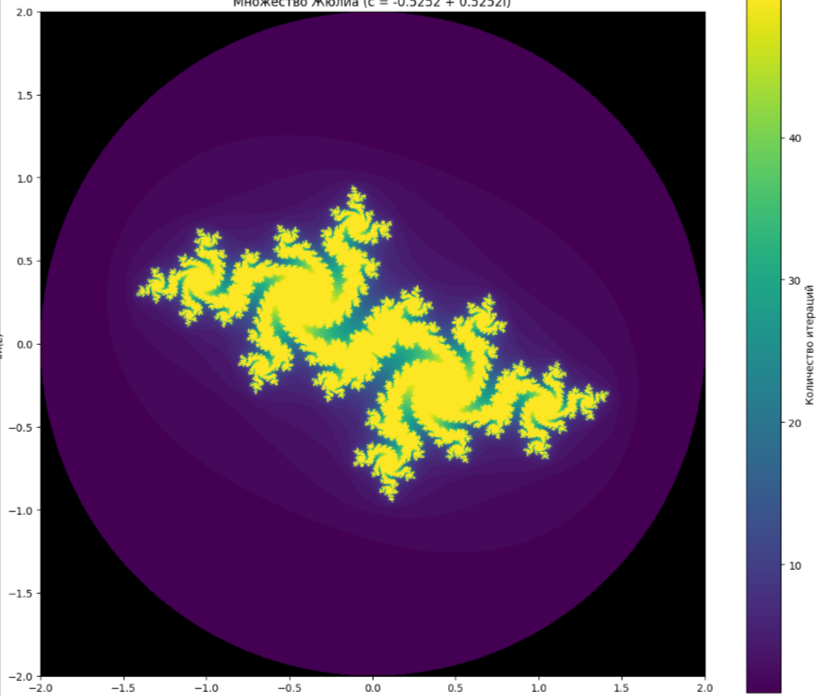
\includegraphics[width=\textwidth]{plots/J3.png}
        \caption{Пример из т/з, 50 итераций}
    \end{subfigure}
    \hspace{1.7cm}
    \begin{subfigure}{0.4\textwidth}
        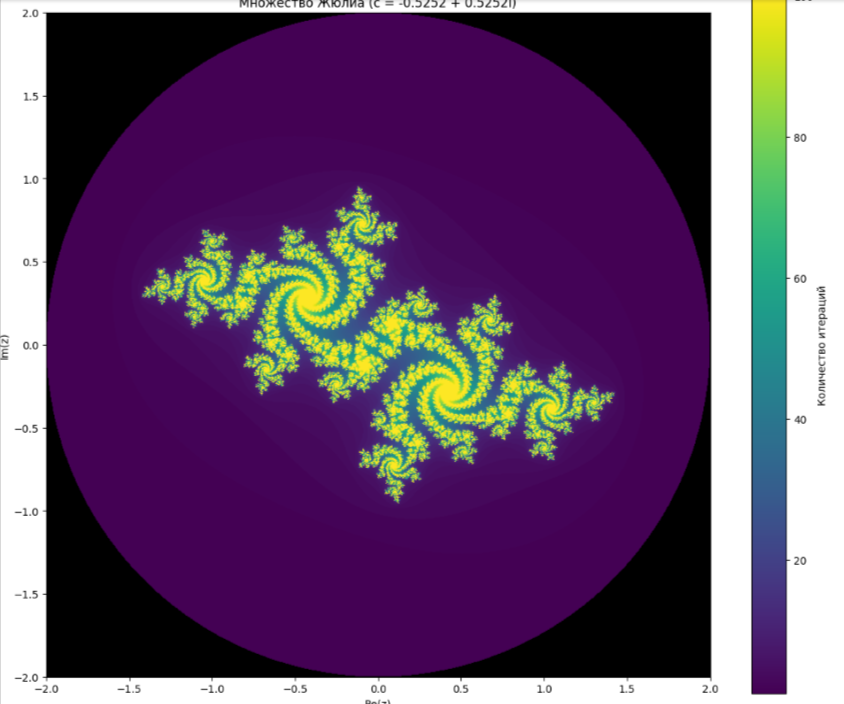
\includegraphics[width=\textwidth]{plots/J4.png}
        \caption{Пример из т/з, 100 итераций}
    \end{subfigure}
    \\
    \begin{subfigure}{0.4\textwidth}
        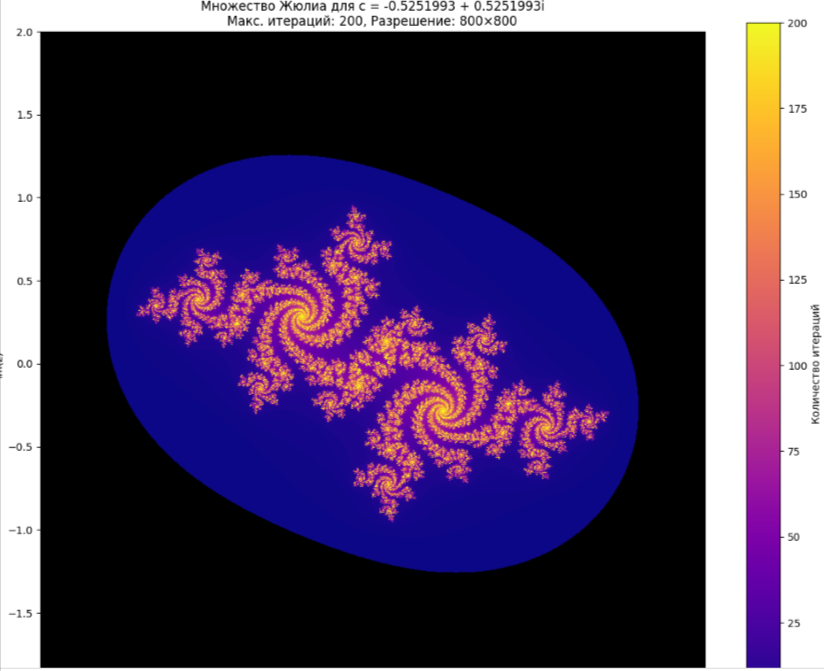
\includegraphics[width=\textwidth]{plots/J1.png}
        \caption{Пример из т/з, 200 итераций}
    \end{subfigure}
    \hspace{1.7cm}
    \begin{subfigure}{0.4\textwidth}
        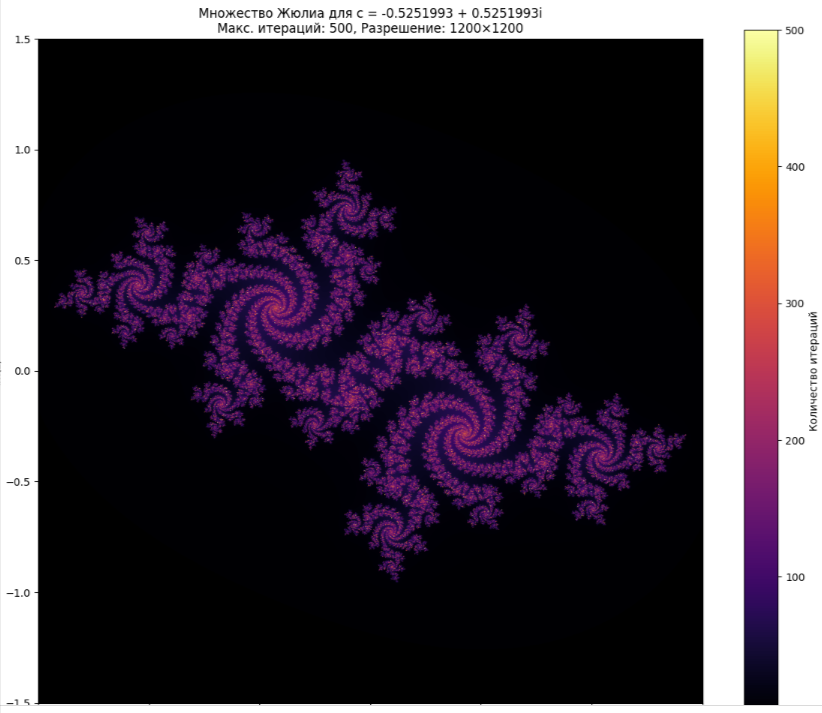
\includegraphics[width=\textwidth]{plots/J2.png}
        \caption{Пример из т/з, 500 итераций }
    \end{subfigure}
    \\
    \caption{примеры при различных С, 100 итераций }
    \hspace{1.7cm}
    \begin{subfigure}{1\textwidth}
        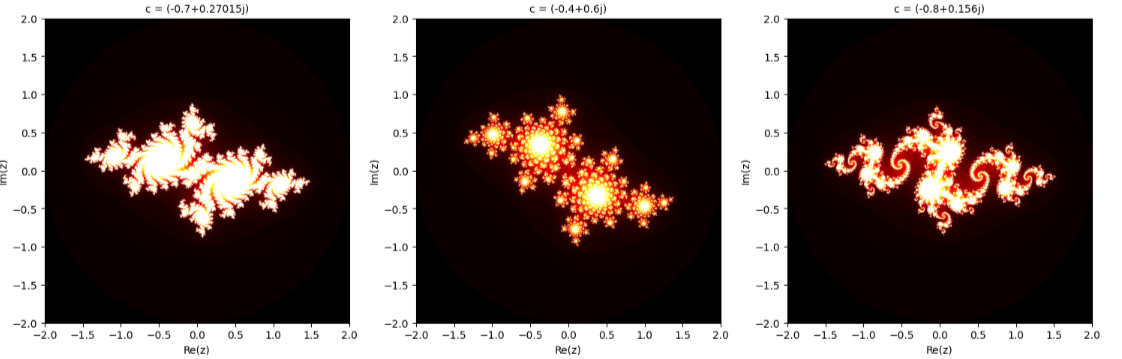
\includegraphics[width=\textwidth]{plots/J5.png}
    \end{subfigure}
    \hspace{1.7cm}
    \begin{subfigure}{1\textwidth}
        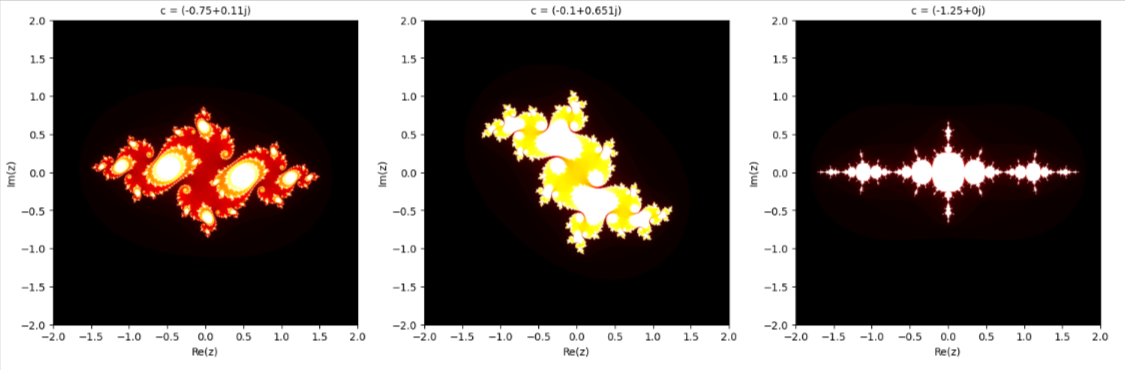
\includegraphics[width=\textwidth]{plots/J6.png}
    \end{subfigure}
\end{figure}